%!TEX root = main.tex

One of the key innovations in \rdfframes is the query generation process.
Query generation produces a \sparql query from an \rdfframe representing a sequence of calls to \rdfframes operators.
The guidelines we use in query generation to guarantee efficient processing are as follows:

\squishlist
\item
Include all of the computation required for generating an \rdfframe in the \sparql query sent to the RDF engine.
Pushing computation into the engine enables \rdfframes to take advantage of the benefits of a database system such as query optimization, bulk data processing, and near-data computing.

\item
Generate one \sparql query for each \rdfframe, never more. \rdfframes combines all graph patterns and operations described by an \rdfframe 
into a single \sparql query.
This minimizes the number of interactions with the RDF engine and enables the query optimizer to explore all optimization opportunities since it can see all operations.

\item
Ensure that the generated query is as simple as possible.
The query generation algorithm generates graph patterns that minimize the use of nested subqueries
and union %operators
\sparql patterns, since these are known to be expensive.
Note that, in principle, we are doing part of the job of the RDF engine's query optimizer.
A powerful-enough optimizer would be able to simplify and unnest queries whenever possible.
However, the reality is that \sparql is a complex language on which query optimizers do not always do a good job. As such, any steps to help the query optimizer are of great use. We show the performance benefit of this approach in Section~\ref{sec:performance}.

\item
Adopt a lazy execution model, generating and processing a query only when required by the user.%needed.

\item
Ensure that the generated \sparql query is correct, that is, ensure the query is semantically equivalent to the \rdfframe. We prove this in Section~\ref{sec:correctness}.

\squishend


\begin{figure}
  \centering
  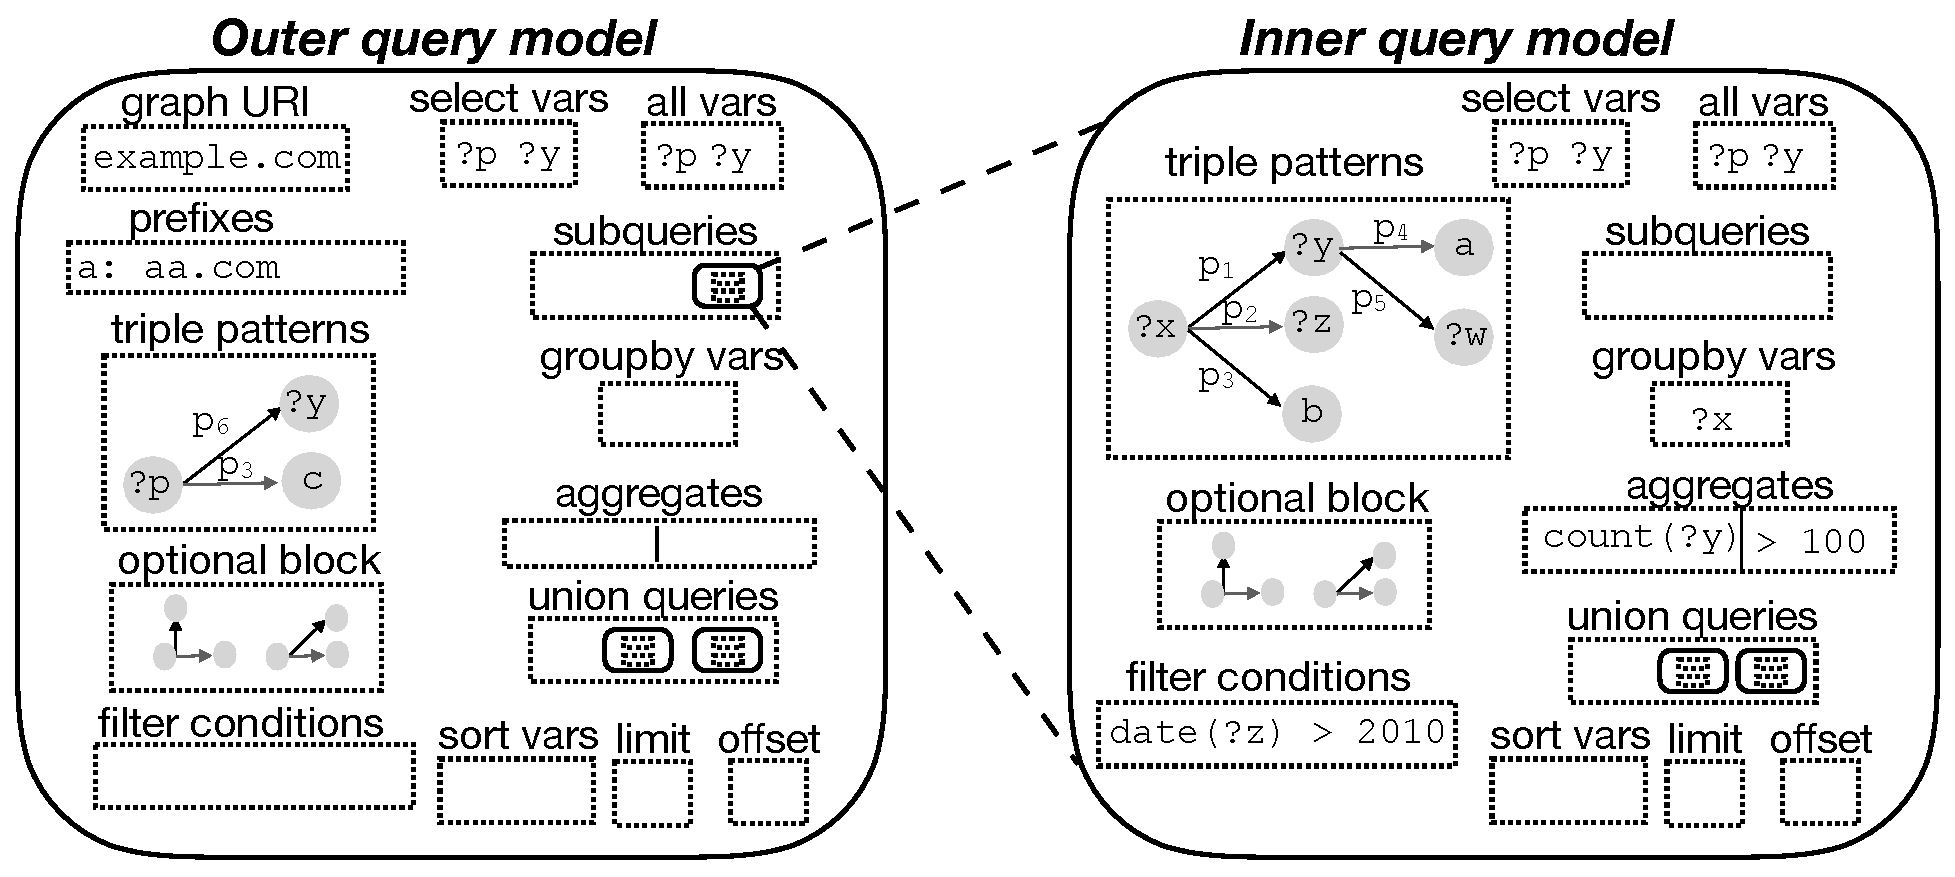
\includegraphics[width=\columnwidth]{figures/querymodel-subquery}
  \caption{Example of an \rdfframes nested query model.}
  \label{fig:querymodel}
  \vspace*{-8pt}
\end{figure}

%Query generation in \rdfframes is a two-step process. First, the sequence of operators describing the \rdfframe is converted to an intermediate representation that we call the {\em query model}. Second, the query model is traversed to generate the \sparql query.
%\subsection{Query Model}

\vspace*{-3pt}
Our query model is inspired by the Query Graph Model~\cite{Pirahesh:1992}, and it
%the query model
encapsulates all components required to construct a \sparql query. 
Query models can be nested in cases where nested subqueries are required.
Using the query model as an intermediate representation between an \rdfframe and the corresponding \sparql query allows for 
(i)~flexible implementation by separating the operator manipulation logic from the query generation logic, and (ii)~simpler optimization.
% by, for example,
%minimizing the number of \sparql query templates that are needed.
Without a query model, a naive implementation of \rdfframes would 
%A naive implementation would 
translate each operator to a \sparql pattern and encapsulate it in a subquery,
with one outer query joining all the subqueries to produce the result.
This is analogous to how some software-generated SQL queries are produced.
Other implementations are possible such as producing a \sparql query for
each operator and re-parsing it every time it has to be combined with a new pattern,
or directly manipulating the parse tree of the query.
The query model enables a simpler and more powerful implementation.

An example query model representing a nested \sparql query is shown in Figure~\ref{fig:querymodel}.
The left part of the figure is the outer query model, which has a reference to the inner query model (right part of the figure). 
The figure shows the components of a \sparql query represented in a query model.
These are as follows:
\squishlist

\item
Graph matching patterns including triple patterns, filter conditions, pointers to inner query models for sub-queries, optional blocks, and union patterns. Graph pattern matching is a basic operation in \sparql.
A \sparql query can be formed by combining triple patterns in various ways using different keywords.
The default is that a solution is produced if and only if
every triple pattern that appears in a graph pattern is matched to the triples in the RDF graph.
The OPTIONAL keyword adds triple patterns that extend the solution if they are matched, but do not eliminate the solution if they are not matched.
That is, OPTIONAL creates left outer join semantics.
The FILTER keyword adds a condition and restricts the query results to solutions that satisfy this condition.

%These patterns are matched to the triples in an RDF graph to extract results. Each pattern in the query model is mapped to the graph it should be matched to.
\item
Aggregation constructs including: group-by columns, aggregation columns, and filters on aggregations (which result in a \texttt{HAVING} clause in the \sparql query). These patterns are applied to the result \rdfframe generated so far. Unlike graph matching patterns, they are not matched to the RDF graph.Aggregation constructs in inner query models are not propagated to outer query models.

\item
Query modifiers including limit, offset and sorting columns.
% with order.
These constructs make final modifications to the result of the query. Any further API calls after adding these modifiers will result in a nested query as the current query model is wrapped and added to another query model. %No further patterns can be added to the query model after adding these modifiers. However, a query model with modifiers can be wrapped in another outer query model.

\item
The graph URIs by the query, the prefixes used, and the variables in the scope of each query.

\squishend

\vspace*{-9pt}
\subsection{Query Model Generation}

\vspace*{-2pt}

%\paragraph{Qeury model generation Algorithm}
The query model is generated lazily, when the special \texttt{execute} function is called
on an \rdfframe.
We observe that generating the query model requires capturing the order of calls to \rdfframes operators and the parameters of these calls, but nothing more.
Thus, each \rdfframe $D$ created by the user is associated with a FIFO queue of operators.
The \texttt{Recorder} component of \rdfframes (recall Figure~\ref{fig:architecture})
%manages this queue and 
records in this queue the sequence of operator calls made by the user.
When \texttt{execute} is called, the \texttt{Generator} component of \rdfframes creates the query model incrementally by processing the operators in this queue in FIFO order.
\rdfframes starts with an empty query model $m$. For each operator pulled from the queue of $D$, its corresponding \sparql component is inserted into $m$. 
Each \rdfframes operator edits one or two components of $m$.
\textit{All of the optimizations to generate efficient \sparql queries are done during query model generation.}
%All the query optimization is done during query model generation. 

The first operator to be processed is always a $seed$ operator for which \rdfframes adds the corresponding triple pattern to the query model $m$. 
To process an $expand$ operator, it adds the corresponding triple pattern(s) to $m$. For example, the operator $expand(x, pred, y, \text{out}, \text{false})$ will result in the triple pattern $(?x, pred, ?y)$ being added to the triple patterns of $m$. Similarly, processing the $filter$ operator adds the conditions that are input parameters of this operator to the filter conditions in $m$.
%the query model.
To generate succinct optimized queries,  \rdfframes adds all triple and filter patterns to the same query model $m$, as long as the semantics are preserved. %the set of triple and filter patterns in one query model $m$. Subsequent patterns are added to the same pre-existing query model as long as the semantics are preserved.
As a special case, when $filter$ is called on an aggregated column, the \texttt{Generator} adds the filtering condition to the $having$ component of $m$. 

One of the main challenges 
%we had to deal with when 
in designing \rdfframes was identifying the cases where a nested \sparql query is necessary. We were able to limit this to %identify
three cases where a nested query is needed to maintain the semantics:
\squishlist
    \item Case 1: when an $expand$ or $filter$ operator has to be applied on a grouped \rdfframe. The semantics here can be thought of as creating an \rdfframe that satisfies the expand or filter pattern and then joining it with the grouped \rdfframe. For example, the \rdfframes code in Listing~\ref{lst:case1_code} expands the \textit{country} column to obtain the \textit{continent} after the \texttt{group\_by} and \texttt{count}. This is semantically equivalent to building an \rdfframe of countries and their continents and then performing an inner join with the grouped \rdfframe.
    \vspace{8pt}
\begin{lstlisting}[
  aboveskip=-0.0\baselineskip,
  belowskip=-0.0\baselineskip,
  language=Python,
  breaklines=true,
  showspaces=false,
  basicstyle=\ttfamily\scriptsize,
  commentstyle=\color{gray},
  otherkeywords={expand, filter, group_by, join, feature_domain_range,entities,  .count, cache, unique},
  keywordstyle=\color{blue},
  caption={\rdfframes code - Expanding a grouped \rdfframe.},
  captionpos=b,
  label={lst:case1_code}]
df = graph.entities(':dpo:Actor', 'actor')\
  .expand('actor', [('dbp:birthPlace', 'country')])\
  .group_by(['actor'])\
  .count('country', 'country_count')\
  .expand('country', [('dbo:continent', 'continent'])
\end{lstlisting}

    \item Case 2: When a grouped \rdfframe has to be joined with another \rdfframe (grouped or non-grouped).
    For example, Listing~\ref{lst:case2_code} represents a join between a grouped \rdfframe and another \rdfframe.
\vspace{8pt}
\begin{lstlisting}[
  aboveskip=-0.0\baselineskip,
  belowskip=-0.0\baselineskip,
  language=Python,
  breaklines=true,
  showspaces=false,
  basicstyle=\ttfamily\scriptsize,
  commentstyle=\color{gray},
  otherkeywords={expand, filter, group_by, join, feature_domain_range,entities, count, cache, unique},
  keywordstyle=\color{blue},
  caption={\rdfframes code - Joining a grouped \rdfframe with another \rdfframe.},
  captionpos=b,
  label={lst:case2_code}]
df1 = graph.entities('dbo:Actor', 'actor')\
  .expand('actor', [('dbp:birthPlace', 'country')])\
  .group_by(['actor']).count('country', 'country_count')
df2 = graph.feature_domain_range('dbp:starring',
  'movie', 'actor').join(df1, 'actor', InnerJoin)
\end{lstlisting}
    \item Case 3: When two datasets are joined by a full outer join.
    For example, the \rdfframes code in Listing~\ref{lst:case3_code}
    is a full outer join between two datasests.
\vspace{8pt}
\begin{lstlisting}[
  aboveskip=-0.0\baselineskip,
  belowskip=-0.0\baselineskip,
  language=Python,
  breaklines=true,
  showspaces=false,
  basicstyle=\ttfamily\scriptsize,
  commentstyle=\color{gray},
  otherkeywords={expand, filter, group_by, join, feature_domain_range,entities, count, cache, unique},
  keywordstyle=\color{blue},
  captionpos=b,
  caption={\rdfframes code - Full outer join.},
  label={lst:case3_code}]
df1 = graph.entities('dpo:Actor', 'actor')\
  .expand('actor', [('dbp:birthPlace', 'country')])
df2 = graph.feature_domain_range('dbp:starring',
  'movie', 'actor').join(df1, 'actor', OuterJoin)
\end{lstlisting}

    %\item Case 2: when a grouped \rdfframe has to be joined with another \rdfframe (grouped or non-grouped).
    %\item Case 3: when two datasets are joined by a full outer join.
    % There is no explicit full outer join between patterns in \sparql so its defined  using the UNION and OPTIONAL ($leftouterjoin$) \sparql patterns instead as the union of the left outer join and the right outer join of $D_1$ and $D_2$.
    There is no explicit full outer join between patterns in \sparql, only left outer join using the OPTIONAL pattern. Therefore, we define full outer join using the UNION and OPTIONAL patterns as the union of the left outer join and the right outer join of $D_1$ and $D_2$.
    %(more details shortly).
    A nesting query is required to wrap the query model for each \rdfframe inside the final query model.
    % except when the join type is full outer join, in which case \sparql \texttt{UNION} is used instead.
\squishend

In the first case, when an $expand$ operation is called on a grouped \rdfframe, \rdfframes has to wrap the grouped \rdfframe in a nested subquery to ensure the evaluation of the grouping and aggregation operations before the expansion. 
\rdfframes uses the following steps to generate the subquery: (i)~create an empty query model $m'$, (ii)~transform the query model built so far $m$ into a subquery of $m'$, and~(iii)~add the new triple pattern from the $expand$ operator to the triple patterns of $m'$. In this case, $m'$ is the outer query model after the $expand$ operator and the grouped \rdfframe is represented by the inner query model $m$. Similarly, when $filter$ is applied on a grouping column in a grouped \rdfframe, \rdfframes creates a nested query model by transforming $m$ into a subquery. This is necessary since the filter operation was called after the aggregation and, thus, has to be done after the aggregation to maintain the correctness of the aggregated values. 


The second case in which a nested subquery is required is when joining a grouped \rdfframe with another \rdfframe.
In the following, we describe in full the different cases of processing the $join$ operator, including the cases when subqueries are required.

To process the binary $join$ operator, \rdfframes needs to join two query models of two different {\rdfframe}s $D_1$ and $D_2$. If the join type is full outer join, a complex query that is equivalent to the full outer join
is constructed using the \sparql
OPTIONAL ($\leftouterjoin$) and UNION ($\cup$) patterns. 
%available in \sparql 
Formally, $D_1 \fullouterjoin D_2 = (D_1 \leftouterjoin D_2)\ \cup \rho_{reorder} (D_2   \leftouterjoin D_1)$.


To process a full outer join, two new query models are constructed: 
The first query model ${m_1}{'}$ contains the left outer join of the query models $m_1$ and $m_2$, which represent $D_1$ and $D_2$, respectively.
The second query model ${m_2}{'}$ contains the right outer join of the of the query models $m_1$ and $m_2$, which is equivalent to the left outer join of $m_2$ and $m_1$. The columns of ${m_2}{'}$ are reordered to make them union compatible with ${m_1}{'}$. Nested queries are necessary to wrap the two query models $m_1$ and $m_2$ inside ${m_1}{'}$ and ${m_2}{'}$.
%in each 
%the new query models . 
%The 
One final outer query model unions the two new query models ${m_1}{'}$ and ${m_2}{'}$.
%The \sparql query that we will  in 
%Listing~\ref{lst:genresparql} is an example of a query that would be generated by this process.
%Listing~\ref{lst:motivating_short_code} is generated using this process.

For other join types, we distinguish three cases:
\squishlist
	\item $D_1$ and $D_2$ are not grouped: \rdfframes merges the two query models into one by combining their graph patterns (e.g., triple patterns and filter conditions). If the join type is left outer join, the patterns of $D_2$ are added inside a single OPTIONAL block of $D_1$. Conversely, for a right outer join the $D_1$ patterns are added as OPTIONAL in $D_2$. No nested query is generated here.
	\item $D_1$ is grouped and $D_2$ is not:
  % (or vice versa):
  \rdfframes merges the two query models via nesting. The query model of $D_1$ is the inner query model, while $D_2$ is set as the outer query model.  If the join type is left outer join, $D_2$ patterns are wrapped inside a single OPTIONAL block of $D_1$, and if the join type is right outer join, the subquery model generated for $D_1$ is wrapped in an OPTIONAL block in $D_2$. This is an example of the second case in which nested queries are necessary. The case when $D_2$ is grouped and $D_1$ is not is analogous to this case.
  % (or vice versa, respectively). 
	\item Both $D_1$ and $D_2$ are grouped: \rdfframes creates one query model containing two nested query models, one for each \rdfframe, another example of the second case where nested queries are necessary. %This is another example of the second case in which nested queries are necessary.
\squishend

If $D_1$ and $D_2$ are constructed from different graphs, the original graph URIs are used in the inner query to map each pattern to the graph it is supposed to match.


To process other operators such as $select\_cols$ and $group\_by$, \rdfframes fills the corresponding component in the query model. The $head$ operator maps to the $limit$ and
%$offset$ 
\textit{offset} components of the query model $m$. To finalize the join processing, \rdfframes unions the selection variables of the two query models, and takes the minimum of the offsets and the maximum of the limits (in case both query models have an offset and a limit).

\vspace*{-9pt}
\subsection{Translating to \sparql}
%\noindent{\textbf{Translating a Query Model into \sparql}}: %\aia{We have to say something about this!}
\begin{sloppypar}
The query model is designed to make translation to \sparql as direct and simple as possible. \rdfframes traverses a query model and translates each component of the model directly to the corresponding \sparql construct, following the syntax and style guidelines of \sparql.
% Each component in the query model is translated to the corresponding \sparql construct. 
For example, each prefix is translated to \texttt{PREFIX name\_space:name\_space\_uri}, graph URIs are added to the \texttt{FROM} clause, and each triple and filter pattern is added to the \texttt{WHERE} clause. The inner query models are translated recursively to \sparql queries and added to the outer query using the subquery syntax defined by \sparql.
When the query accesses more than one graph and different subsets of graph patterns are matched to different graphs, the \texttt{GRAPH} construct is used to wrap each subset of graph patterns with the matching graph URI. 
\end{sloppypar}

The generated \sparql query is sent to the RDF engine or \sparql endpoint using 
the \sparql protocol\footnote{\url{https://www.w3.org/TR/sparql11-protocol}} over HTTP.
We choose communication over HTTP since it is the most general mechanism to communicate with RDF engines and the only mechanism to communicate with \sparql endpoints.
One issue we need to address is paginating the results of a query, that is, retrieving them in chunks. There are several good reasons to paginate results, for example, avoiding timeouts at \sparql endpoints and bounding the amount of memory used for result buffering at the client. When using HTTP communication, we cannot rely on RDF engine cursors to do the pagination as they are engine-specific and not supported by the \sparql protocol over HTTP. The HTTP response returns only the first chunk of the result and the size of the chunk is limited by the \sparql endpoint configuration. The \sparql over HTTP client has to ask for the rest of the result chunk by chunk but this functionality is not implemented by many existing clients. %pagination is done by issuing the query multiple times using different LIMIT and OFFSET values.
Since our goal is generality and flexibility, \rdfframes implements pagination 
transparently to the user and returns one dataframe with all the query results.